\IEEEraisesectionheading{\section{Introduction}
\label{sec:Introduction}}
%\IEEEPARstart{S}{oftware} defect prediction is one of the most active research areas in
%software
%engineering (SE)~\cite{DAmbros12,Fukushima14,Lee11,Lessmann08,Li12,Menzies07,Nam13,Rahman12,Shivaji13,Zimmermann08,Zimmermann09}.
%If software quality assurance teams can predict defects before releasing a
%software product, they can effectively allocate limited
%resources for quality control~\cite{Menzies07,Ostrand05,Rahman12,Zimmermann08}.
%For example, Ostrand et al. applied defect prediction in two large software systems
%of AT\&T for effective and efficient testing activities~\cite{Ostrand05}.
% For
% this reason, many software defect prediction studies have been
%conducted~\cite{DAmbros12,Lee11,Lessmann08,Li12,Mende10,Menzies07,Shivaji13,Zimmermann08}.

\IEEEPARstart{M}{achine} learners can be used to automatically generate software quality
models from project data~\cite{DAmbros12,Menzies07}. 
Such data comprises  various {\em software metrics} and {\em labels}:
\squishlist
\item
{\em Software metrics} are the terms used to describe software projects. Commonly
used software metrics for defect prediction are complexity metrics (such as lines of code, Halstead
metrics, McCabe's cyclometic complexity, and CK metrics) and
process metrics~\cite{Basili96,Halstead77,McCabe76,Rahman13}.
\item
When learning defect models,
{\em labels} indicate
whether the source code is buggy or clean for binary
classification~\cite{Lee11,Nam13}.
\squishend
% These metrics measure how software and its development process are complex, and
% they are used as features for building a prediction model based on machine
% learning.

\noindent
Most proposed defect prediction models have been evaluated on
``within-project'' defect prediction (WPDP)
settings~\cite{DAmbros12,Lee11,Menzies07}.
As shown
in Figure~\ref{fig:subfig1}, in WPDP,  each instance representing a source code file or
function consists of software metric values and is labeled as buggy or clean.
In the WPDP setting, a prediction model is
trained using the labeled instances in {\em Project A} and predict unlabeled (`?')
instances in the same project as buggy or clean.

It is difficult to build a prediction model for new
software projects or projects with little historical
information~\cite{Zimmermann09} since such projects lack sufficient training
data. 
%Various process metrics and label information can be extracted from
%the historical data of software repositories such as version control and issue
%tracking systems~\cite{Rahman13}.
%Thus, it is difficult to collect process metrics and instance
%labels in new projects or projects that have little historical
%data~\cite{Fukushima14,Nam13,Zimmermann09}. For example, without instances being
%labeled using past defect data, it is not possible to build a prediction model.
%~\sung{Here your
%supporting sentences are weak and your argument is not so convincing. Any more
% backup or citations?}
To address this issue, researchers
have proposed ``cross-project'' defect
prediction (CPDP)~\cite{He12, Ma12, Nam13, Rahman12, Turhan09, Zimmermann09}.
CPDP approaches predict defects even for new projects lacking
in historical data by reusing information from other projects. As shown in Figure~\ref{fig:subfig2}, in CPDP,
a prediction model is trained by
labeled instances in {\em Project A} (source) and predicts defects in {\em Project B} (target).

%\sung{This part is not relevent, since you are not improving cross-defect prediction.}
% The cross-prediction  has been a challenging issue because of
% its poor prediction performance~\cite{Turhan09,Zimmermann09}.
% For example, Zimmermann et al. conducted 622 cross-predictions but only 3.4\%
% cross-predictions worked~\cite{Zimmermann09}.
% 
% To improve cross-prediction performance, many
% attempts have been made~\cite{Ma12,Nam13,Turhan09,Watanabe08}.
% In our previous study, transfer defect learning~\cite{Nam13}, we proposed a
% novel approach, TCA+, and showed the performance of cross-project defect prediction is
% comparable with within-project prediction in our experimental settings.
% Studies by Briand et al.~\cite{Briand02} and Rahman et al.~\cite{Rahman12} found
% that the cross-prediction is viable in terms of cost-effectiveness.

Most CPDP approaches have a serious limitation:
typical CPDP requires that all projects collect exactly the same metrics (as shown Figure~\ref{fig:subfig2}). Finding other projects with exactly
the same metric set can be challenging. Publicly available defect
datasets that are widely used in defect prediction literature usually have
{\em heterogeneous} metric sets:
\squishlist
\item

In   heterogenous data, different metrics are collected in different projects.
\item
For example, many NASA datasets in the PROMISE repository have 37 metrics but
AEEEM datasets used by D'Ambros et al. have 61
metrics~\cite{DAmbros12,promise12}.
The only common metric between NASA and AEEEM datasets is {\em lines of
code (LOC)}.
CPDP between NASA and AEEEM
datasets with all metric sets is not feasible since they have
completely different metrics~\cite{Turhan09}.
\squishend
% Different metric sets among project datasets are due to different
% development `contexts' such as programing language, open-/closed-source, 
% application domain, system size, and etc.~\cite{Zhang13}. For
% example, we cannot extract the object-oriented metrics from the software
% projects that are not developed in object-oriented languages. In case of
% proprietary project datasets such as NASA and SOFTLAB widely
% used in defect prediction studies~\cite{Ma12,Turhan09}, we can only use
% publicly available metrics since we can not collect other kinds of metrics as
% companies are reluctant to make their software repositories publicly available.
% In addition, metric values may have different distributions in different development environments.
% Zhang et al. considered
% difference of development environments as several context factors and analyzed
% that the context factors affect the distribution of software
% metrics~\cite{Zhang13}.
Some CPDP studies use only common metrics when source and target datasets have
heterogeneous metric sets~\cite{Ma12,Turhan09}.
For example, Turhan et al. use the only 17 common metrics between the NASA and
SOFTLAB datasets that have heterogeneous metric sets~\cite{Turhan09}. 
This approach is hardly a general solution since
finding other projects with multiple common metrics can be challenging. As
mentioned, there is only one common metric between NASA and AEEEM. Also,
only using common metrics may degrade the performance of CPDP models.
That is because some informative metrics necessary for building a good prediction model may not
be in the common metrics across datasets. For example, the CPDP approach proposed by Turhan et al. did not
outperform WPDP in terms of the average
f-measure (0.35 vs. 0.39)~\cite{Turhan09}.
% In addition, metric values among
% projects developed in different development contexts can have different
% distributions as in the study by Zhang et al.~\cite{Zhang13}. This can lead to
% the poor prediction results in CPDP~\cite{Pan10}. For example, in the study of
% Nam et al., before applying their TCA+ that tries to make different distributions of source and
% target metric values similar, the average f-measure (0.35) of CPDP without TCA+
% was significantly worse than that (0.45) of CPDP with TCA+~\cite{Nam13}.

% This limitation
% is revealed in three types in most cross defect prediction research papers.
% The first type is that all datasets with the same
% feature space were newly collected for their cross prediction study. Studies by
% Zimmermann et al.~\cite{Zimmermann09} and Rahman et al.~\cite{Rahman12} belong
% to the first type. Collecting new datasets can prevent active works for cross
% prediction studies because of enormous efforts mining and labeling data.
% 
% The second type is that only common features (metrics) across existing datasets
% are used to training and test a prediction model as in Turhan et al.'s
% study~\cite{Turhan09}. ReLink dataset used in our previous study also used
% common features among three datasets~\cite{Nam13}. This type may degrade the
% performance of defect prediction models because some informative features
% necessary for building a good prediction model can be excluded in common
% features across datasets.
% 
% The third type is that cross defect prediction was conducted only within
% a group of datasets having the same feature space~\cite{Nam13}. This hinders to
% flexibly apply cross prediction techniques in practice since the pool of
% datasets with the same feature space for defect prediction is confined although
% there are lots of existing datasets available. In our previous study, we
% used two groups of datasets, ReLink and AEEEM~\cite{Nam13}. However, we could
% not conduct cross-project defect prediction between ReLink and AEEEM because of the
% different feature spaces. As explained in three types, cross prediction research
% was evaluated only with newly collected or confined datasets with the same
% feature space.


% 
% If it is possible to conduct CPDP on datasets with
% different metric sets as in Figure~\ref{fig:subfig3}, we could actively reuse
% existing abundant defect datasets to build a prediction model. For example, most
% PROMISE defect datasets even if they have different metrics~\cite{promise12}
% could be used as training datasets. This might be really helpful to improve the
% performance of defect prediction models.



% Recently, many researchers on machine learning have actively focused on
% studies regarding transfer learning since reusing existing datasets can reduce
% costs for building better machine learning models~\cite{Pan10}. In this sense,
% our study for the software engineering research also follows the transfer
% learning discipline.

% The goal of this study is to investigate the possibility to build good
% cross-domain defect prediction models by using datasets with different feature
% spaces.

In this paper, we propose the heterogeneous defect prediction (HDP) approach
to predict defects across projects even with heterogeneous metric
sets.
If the proposed approach is feasible as in
Figure~\ref{fig:subfig3}, we could reuse any existing defect
datasets to build a prediction model. For example, many PROMISE defect datasets
even if they have heterogeneous metric sets~\cite{promise12} could be used as
training datasets to predict defects in any project.

The key idea of our HDP approach is to transfer knowledge from a source dataset to predict defects in a target dataset by matching metrics that have
similar distributions between source and target datasets. In addition, we also
used metric selection to remove less informative metrics of a source dataset
for a prediction model before metric matching.

In addition to proposing HDP, it is important to identify the lower bounds of the sizes of the source and target datasets for effective transfer learning since HDP compares distributions between source and target datasets. 
%However, when conducting HDP, there is another issue, "how early can we transfer knowledge from source to target?"
If HDP requires many source or target instances to compare there distributions, HDP may not be effective and efficient to build a prediction model. We address this limit experimentally as well as theoretically in this paper.


\begin{figure}[t]

	\centering
 
 \begin{subfigure}[b]{0.8\linewidth}
 	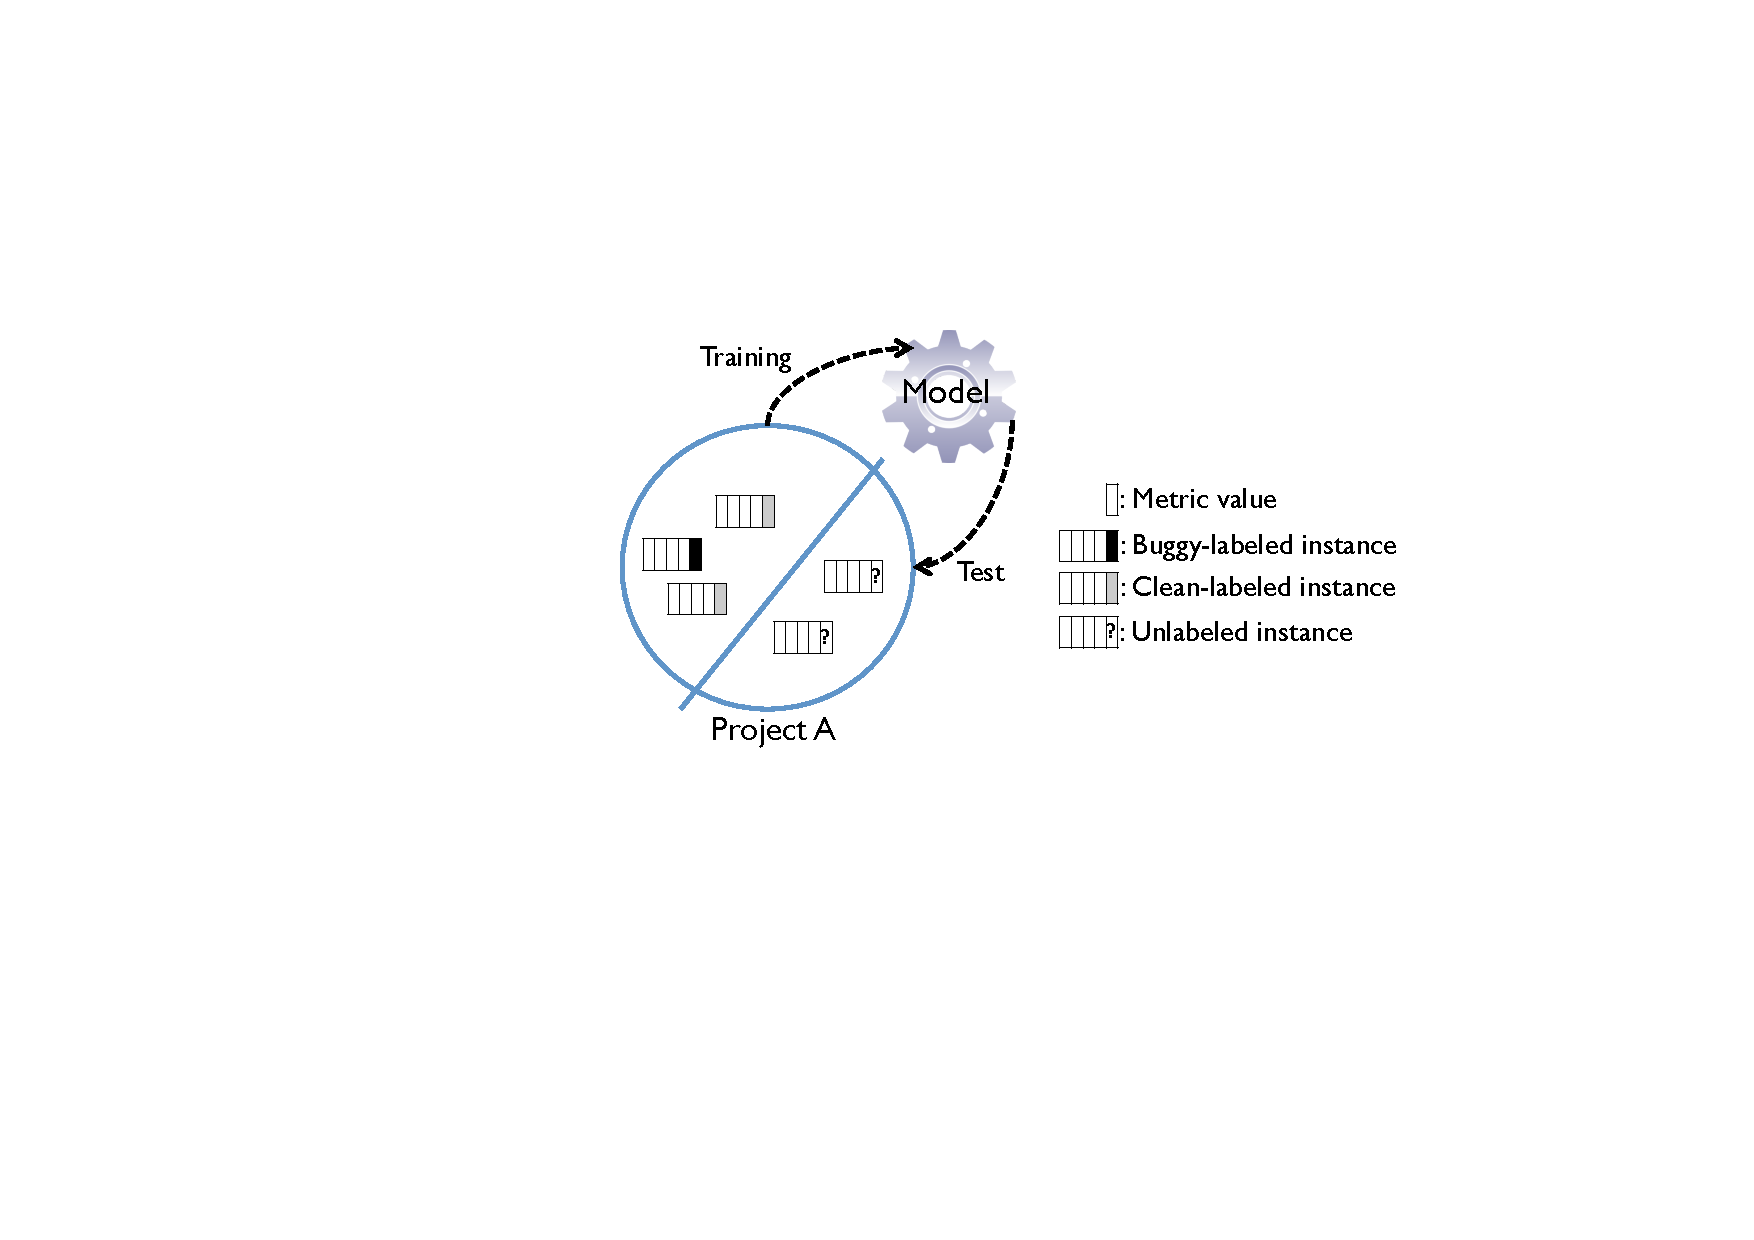
\includegraphics[scale=0.5]{Figures/intro/p_within.pdf}
  	\caption{Within-Project Defect Prediction \tiny{(WPDP)}}
   	\label{fig:subfig1}
 \end{subfigure}
 
 \begin{subfigure}{0.8\linewidth}
 	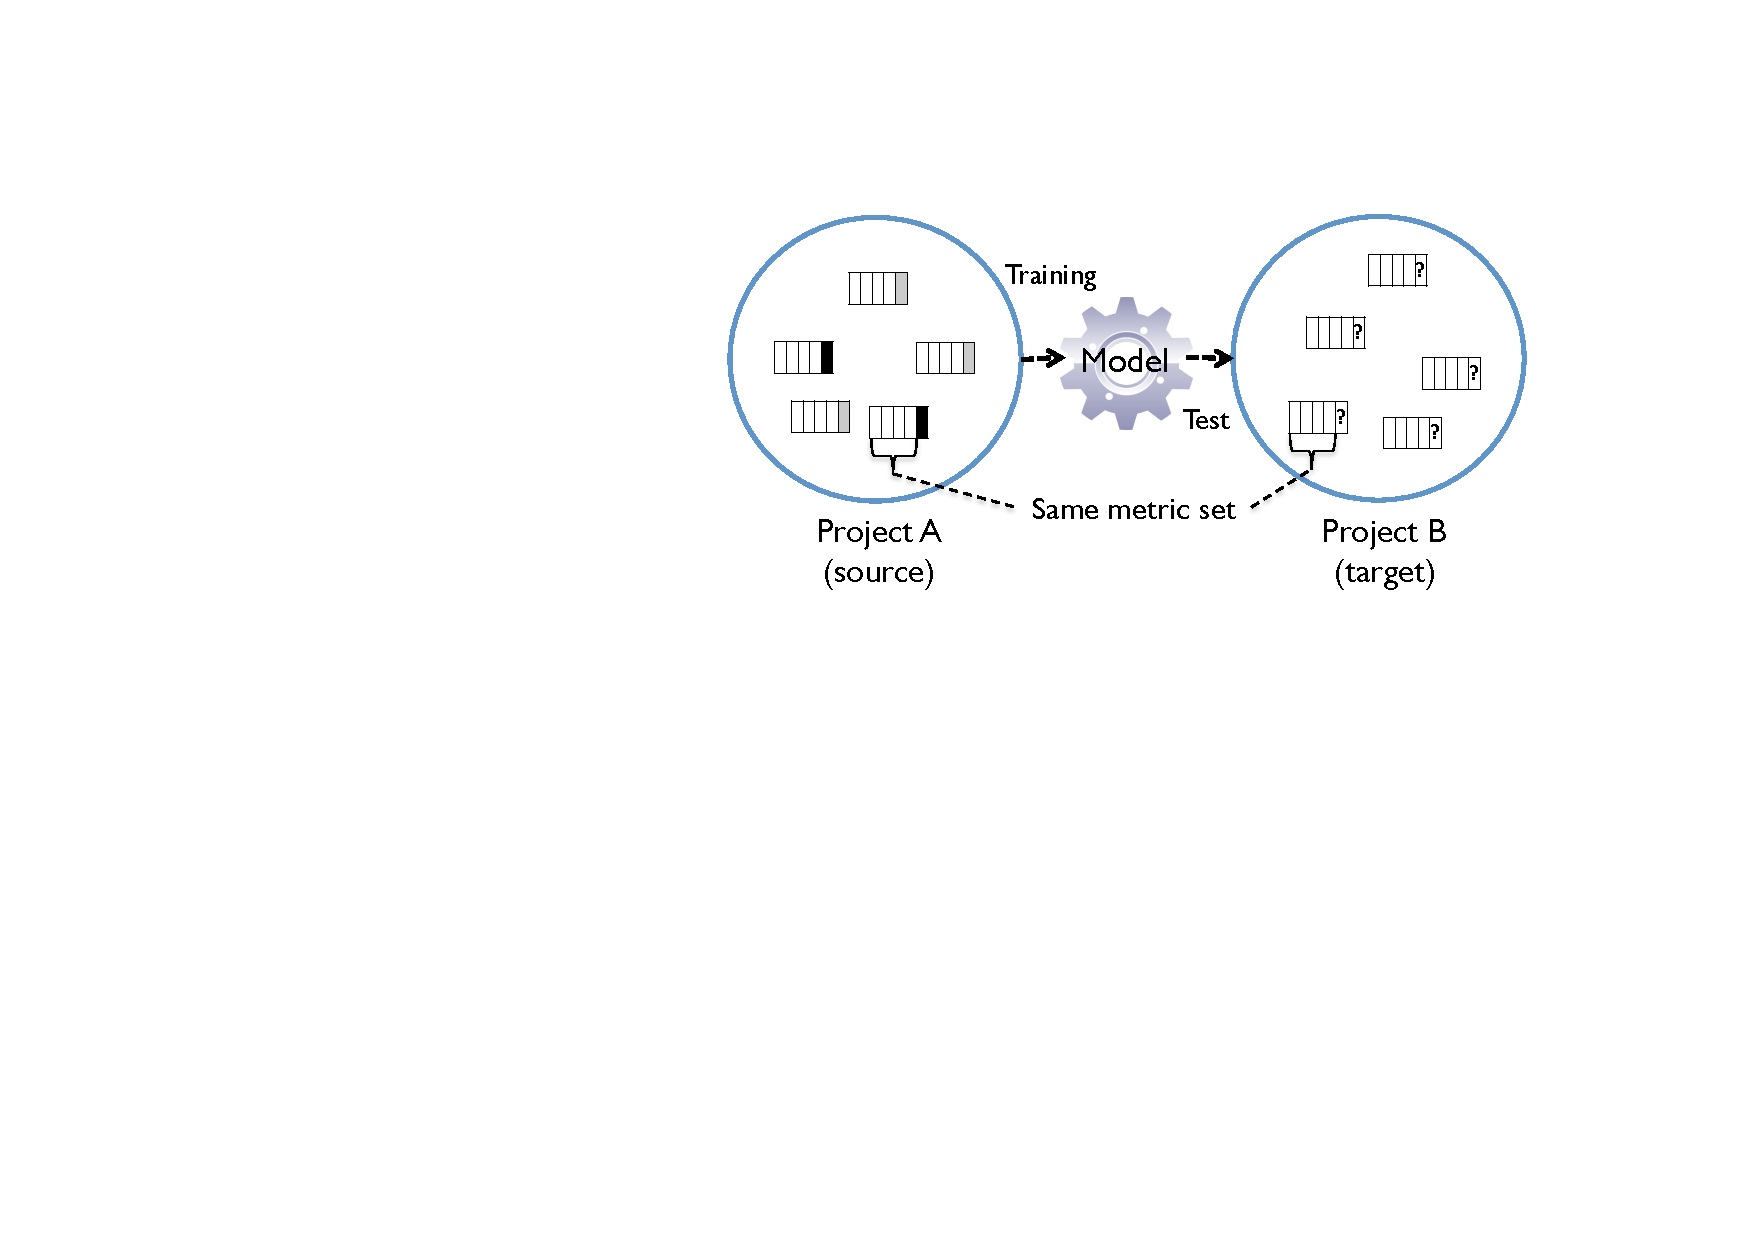
\includegraphics[scale=0.5]{Figures/intro/p_cross.pdf}
  	\caption{Cross-Project Defect Prediction \tiny{(CPDP)}}
   	\label{fig:subfig2}
 \end{subfigure}
 
 \begin{subfigure}{0.8\linewidth}
 	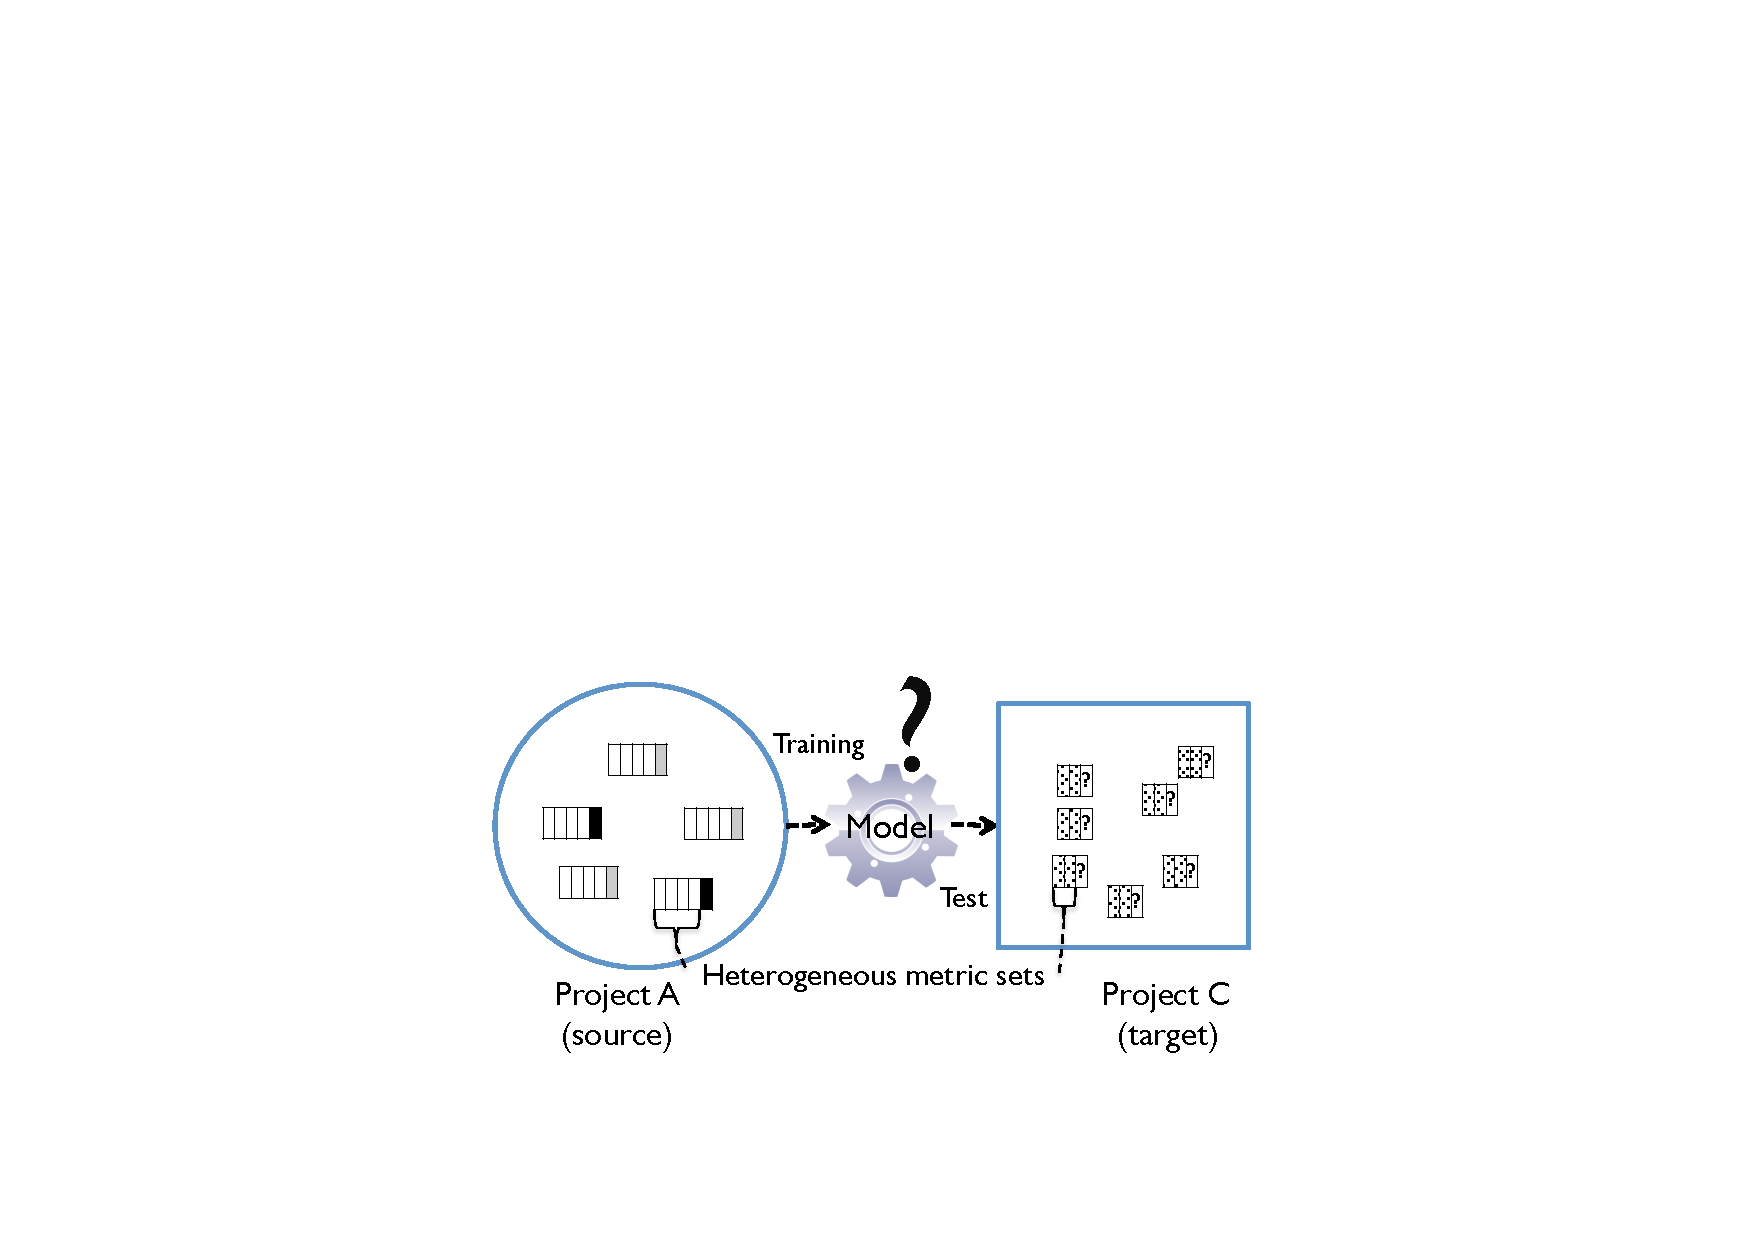
\includegraphics[scale=0.5]{Figures/intro/p_crossdomain.pdf}
  	\caption{Heterogeneous Defect Prediction \tiny{(HDP)}}
   	\label{fig:subfig3}
 \end{subfigure}
 
 \label{fig:type_of_predictions}
 \caption{%
  %Caption of subfigures \subref{fig:subfig1}, 
  %\subref{fig:subfig2} and \subref{fig:subfig3}
  Various Defect Prediction Scenarios
  }
\end{figure}

\subsection{Research Questions}
To systematically evaluate HDP models, we set
two research questions.
\squishlist
  \item RQ1: Is heterogeneous defect prediction comparable to WPDP and existing CPDP approaches for heterogeneous metric sets?
   \item RQ2: What are the  lower  bounds  of  the  size  of source and target  datasets  for  effective HDP?
%   \item[RQ2:] Are cross-domain defect predictions from non-defect to
%   defect datasets comparable to within-predictions?
%  \item[RQ3:] What is the prediction coverage of cross-domain defect
%  prediction?
\squishend
% 
% Since we designed four feature matching analyzers, we identify the
% best co-occurrence analyzers among the five analyzers introduced in
% Section~\ref{sec:analyzers} (RQ1).

\subsection{Contributions}
Our experimental study shows that HDP models are feasible and their prediction
performance is promising. About 50\% -- 74\% of HDP predictions
are better or comparable to predictions in baseline approaches with statistical
significance.


For RQ2, we conducted the experimental study by using various sampling sizes of source and target datasets for HDP and validate the generality of its results through a {\em Monte Carlo} simulation. Our results suggest that 200 instances for source (with at least 20 defective samples) and target datasets could be effective enough for our HDP models.


% To our knowledge, this is a first study on defect prediction using
% datasets with different feature spaces. We hope this study will suggest a
% promising next step for defect prediction research.

Our contributions are summarized as follows:
\squishlist
  \item Proposing the heterogeneous defect prediction models.
  \item Conducting extensive and large-scale experiments to evaluate
  the heterogeneous defect prediction models.
  \item Validating the lower bounds of the size of source and target datasets for effective heterogeneous defect prediction.
\squishend


\subsection{Extensions from Prior Publication}

We extend the previous conference paper of the same name~\cite{Nam15HDP} in the following ways. First, we motivate this study in the view of transfer learning in software engineering (SE). Thus, we discuss how transfer learning can be helpful to understand the nature of generality in SE and why we focus on defect prediction in terms of transfer learning (Section~\ref{sec:Motivation}). Second, we address new research question about the effective sizes of source and target datasets when conducting HDP.  In Section~\ref{sec:sizelimit} and~\ref{sect:xplain}, we show experimental and theoretical validation to investigate the effective sizes of project datasets for HDP. Third, we discuss more related work with recent studies. In Section~\ref{sec:Background}, we discuss metric sets used in CPDP and how our HDP is similar to and different from recent studies about CPDP using heterogeneous metric sets.
%Fourth, we conduct the effect size analysis using Cliff's $\delta$ to investigate the magnitude of performance improvement by HDP in Section~\ref{sec:Result}.

% This paper is organized as follows. Section~\ref{sec:Background} explains
% the background of our study. % for our framework for cross-domain defect
% % prediction.
% Section~\ref{sec:Approach} presents our HDP model in detail.
% Section~\ref{sec:Evaluation} describes the design of our empirical study. Our
% evaluation results are reported in Section~\ref{sec:Result}. In
% Section~\ref{sec:Discussion}, we discuss insights of our results as well as
% threats to validity. Section~\ref{sec:Conclusion} summarizes and concludes our
% study.


